% !TeX spellcheck = en_US
\section{Neural Network Architecture}
In the evolving landscape of NLP, the adaptation of Convolutional Neural Networks on various domains of processing and classification, has marked a significant technological advancement. This transition underscores the versatility of CNNs, which, despite their visual data origins, excel in deciphering the intricate patterns of textual information. The project in discussion exemplifies this innovative application, employing a CNN to tackle a multiclass text classification challenge. Herein, we delve into the architectural choices and strategic decisions underlying the model's design, offering a comprehensive understanding of its construction and functionality. \\
A universal question is wether we must use CNN's or RNN's. The choice between a Convolutional Neural Network (CNN) and a Recurrent Neural Network (RNN) depends on the specific task and the nature of our data. \\

In general, RNN is a class of artificial neural network where connections between nodes form a directed graph along a sequence. It is basically a sequence of neural network blocks that are linked to each other like a chain. Each one is passing a message to a successor. This architecture allows RNN to exhibit temporal behavior and capture sequential data which makes it a more ‘natural’ approach when dealing with textual data since text is naturally sequential. RNNs usually are good at predicting what comes next in a sequence\\

Controversely, CNN is a class of deep, feed-forward artificial neural networks where connections between nodes do not form a circle. CNNs are basically just several layers of convolutions with nonlinear activation functions like ReLU or tanh applied to the results. In a traditional feedforward neural network we connect each input neuron to each output neuron in the next layer. That’s also called a fully connected layer. In CNNs we don’t do that. Instead, we use convolutions over the input layer to compute the output. This results in local connections, where each region of the input is connected to a neuron in the output. Each layer applies different filters, typically hundreds or thousands like the ones shown below, and combines their results. CNNs can learn to classify a sentence or a paragraph.\\

An RNN is trained to recognize patterns across time, while a CNN learns to recognize patterns across space. The best way to determine which to use is to try both and see which one performs better on our project. \\
A big argument for CNNs is that they are exceptionaly fast. Based on computation time, CNN's seems to be much faster, sometimes also 5 times faster, than RNN's.

\begin{figure}[htpb]
	\centering
	\begin{subfigure}{0.47\linewidth}
		\centering
		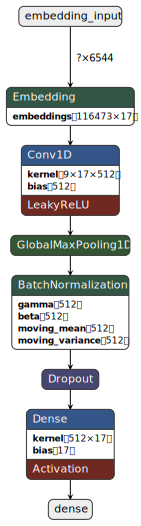
\includegraphics[height=0.9\textheight]{Images/model_level_1.keras.pdf}
		\caption{\textit{category\_level\_1}}
	\end{subfigure}
	\begin{subfigure}{0.47\linewidth}
		\centering
		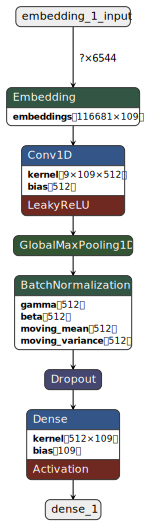
\includegraphics[height=0.9\textheight]{Images/model_level_2.keras.pdf}
		\caption{\textit{category\_level\_2}}
	\end{subfigure}
	\caption{Architecture of the neural networks}
	\label{fig:nn_architectures}
\end{figure}
 
%\begin{minipage}{0.47\linewidth}
%	\centering
%	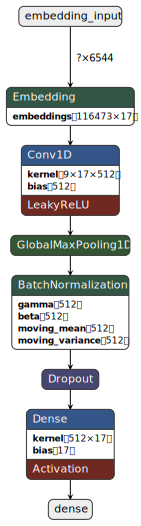
\includegraphics[height=0.9\textheight]{Images/model_level_1.keras.pdf}
%	\captionof{figure}{Architecture of the model for \textit{category\_level\_1}}
%\end{minipage}\hfill
%\begin{minipage}{0.48\linewidth}
%	\centering
%	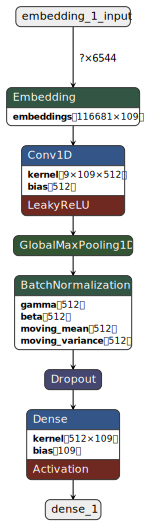
\includegraphics[height=0.9\textheight]{Images/model_level_2.keras.pdf}
%	\captionof{figure}{Architecture of the model for \textit{category\_level\_2}}
%\end{minipage}

\subsection{Embedding Layer}
The embedding layer is a critical component in the neural network architecture, serving as the foundational layer that deals directly with the text input. In the general context of NLP and deep learning, an embedding layer effectively translates tokenized and sequenced text data into dense vectors of fixed size. This layer maps each word to a high-dimensional space where words with similar meanings are located in proximity to one another, thereby capturing semantic relationships in a way that is not possible with sparse representations such as one-hot encoding.

From Figure~\ref{fig:nn_architectures}, we can see that embedding layer has been configured with a vocabulary size of $\num{129865}$ and an output dimension of $17$ for \verb|category_level_1| and of $109$ for \verb|category_level_2|. Those numbers are not set by a random factor, but they represent the number of unique labels in each category. By applying this very specific number (\textit{which changes with different input}), we are sure that our model will compute the correct probability distribution output for the given input data. This setup suggests that our model is designed to handle a large corpus with a rich vocabulary, transforming each token into a $x$-dimensional vector. The decision to use such an embedding size balances the need for a nuanced representation of the input text against the computational efficiency of the model. A smaller dimensionality in the embedding space ensures that the model remains computationally tractable, while still allowing for a meaningful representation of words.

Moreover, the embedding layer is paramount when working with sequences of different lengths. After tokenizing, padding, and converting texts into sequences, the embedding layer takes these sequences as input and provides a uniform output shape, which is essential for the subsequent convolutional layers to function correctly. Unlike one-hot encoded vectors that are sparse and high-dimensional, the dense embeddings can capture more information in a lower-dimensional space.

Thus, by choosing to implement an embedding layer, our model is able to learn an internal representation for the words in the dataset during training. This is advantageous over using pre-trained embeddings when the text data has unique contextual meanings or when the domain-specific vocabulary may not be well-represented by pre-trained word vectors. It allows the model to adapt the word representations to the nuances of the specific dataset and task at hand.


\subsection{Conv1D Layer}
The inclusion of a convolutional layer with a kernel size of $20$ and $512$ filters in the neural network architecture is a calculated choice tailored for the demands of text classification tasks. The kernel size, or filter size, determines the width of the convolution window that scans across the input data. In this case, a kernel size of $20$ allows the model to examine twenty adjacent words at a time, enabling the capture of context within these word sequences. This can be particularly effective for recognizing patterns or features in text that span multiple words, such as phrases or specific syntactic constructions, which are often pivotal for understanding the overall meaning and sentiment of the text.

The use of $512$ filters within this layer significantly increases the model's capacity to extract features. Each filter can be thought of as a feature detector, looking for different types of patterns in the text. With $512$ filters, the network is well-equipped to identify a wide array of textual features, making it robust in the face of the complexity and variability inherent in natural language. This high number of filters is indicative of the model's deep architecture, designed to handle the intricate task of classifying texts into multiple categories, where a nuanced understanding of the language is crucial.

Furthermore, the choice of the \verb|Leaky ReLU| activation function following the convolutional layer adds an element of non-linearity to the model, allowing for more complex relationships to be learned. \verb|LeakyReLU| is particularly chosen over the standard \verb|ReLU| to mitigate the issue of neurons \say{dying} during training; it allows a small, non-zero gradient when the unit is not active, thus maintaining a gradient flow even for neurons that output negative values. This can lead to more efficient learning and better performance, especially in deeper networks that are prone to saturation and dead neurons.

